

% Символы, специфичные для моей статьи по теории возможностей

\newcommand{\td}{т.\,д.}
\newcommand{\te}{т.\,е.}

\title[Выбор объектов по экспертным оценкам]{Выбор наиболее качественных объектов на основе нечётких данных об их характеристиках}
\institute{Физический факультет МГУ имени~М.\,В.\;Ломоносова\\Кафедра информатики и чего-то там}
\author{Борисов Кирилл Александрович}
\date{15 ноября 2015~г.}
% \date{\today}

\begin{document}
\selectlanguage{russian}
\sloppy

\maketitle

\section{Задача выбора объектов}


\begin{frame}{Модель объектов и экспертной оценки}
	%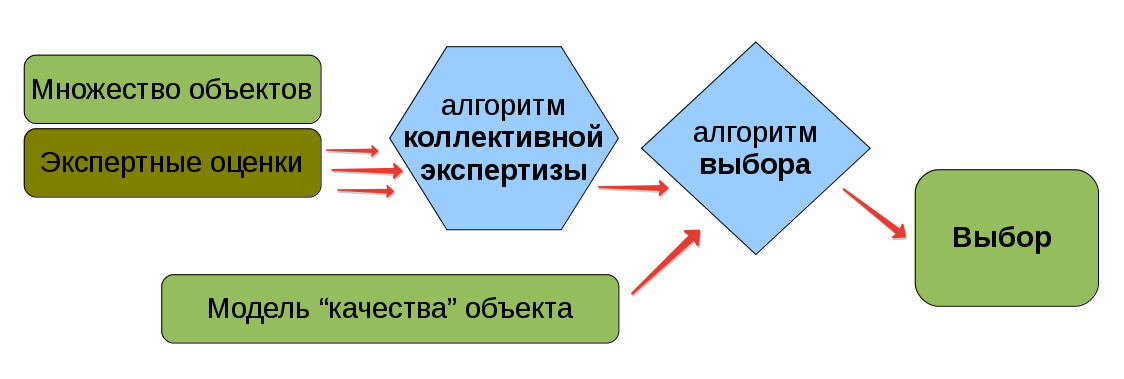
\includegraphics[width=0.8\linewidth]{./pic/globalscheme}
 	\begin{columns}
 		\column{0.45\textwidth}
 			Есть $n$ объектов, у каждого объекта % составителем методологии выбрано
 			есть $m$ нечётких параметров: 
			\\ \vspace*{2mm}
 			$\tilde x_{ij} \in X$, {\footnotesize $i = 1 \ldots n$, $j = 1 \ldots m$} 
 			\\ \vspace*{3mm}
 			$x_{ij} \in X$ -- их значения (неизвестны), где $X$ --  числовое множество. %некое выпуклое подмножество действительной оси
 		\column{0.55\textwidth}
 			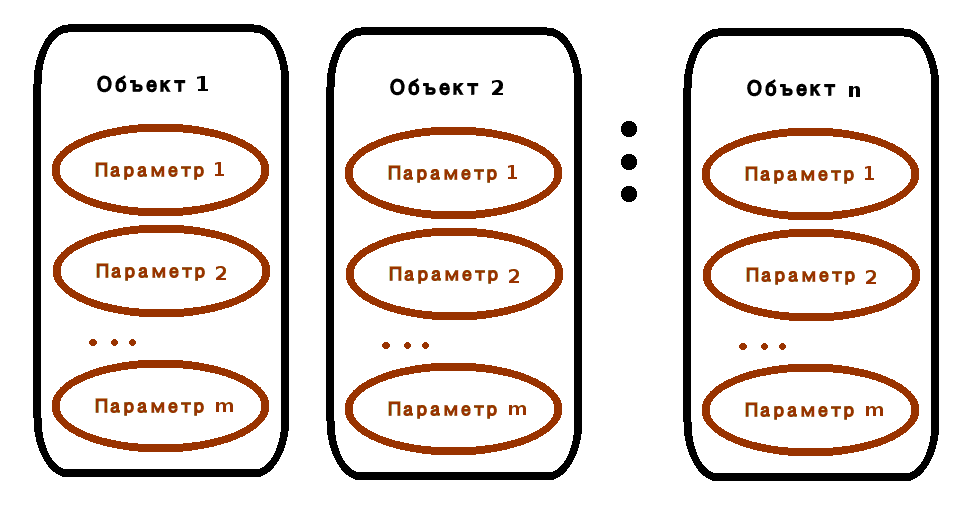
\includegraphics[width=1.0\linewidth]{./pic/theobjects}
 	\end{columns}
 	
        \hspace{20mm} { \small \tikz { \node  (n1) { \light{монотонна и задана заказчиком экспертизы}  }; } }
	 $x_i = \tikz[baseline] { \node[anchor=base, fill=green!20] (t1) {$f$}; } (x_{i1}, ..., x_{im})$ -- <<качество>> объектов.
	\begin{tikzpicture}[overlay]
	    \path[->] (n1.west) edge  (t1.north east);
	\end{tikzpicture}

	\vspace*{3mm}
	\begin{columns}
		\column{0.60\textwidth}
		Экспертные оценки -- это распределения 
		{\large \begin{center} \hspace{-20mm}  $\{ \p_{ij}(x_{ij}) \}_r$ \end{center} }
		{\footnotesize где $i = 1 \ldots n$ -- номер объекта, $j = 1 \ldots m$, -- номер параметра, $r = 1 \ldots R$ -- номер эксперта}.  
		\column{0.40\textwidth}
	\end{columns}
 	
\end{frame} %===========================

\begin{frame}{Пример формирования <<качества>> объекта}
	\begin{center}
		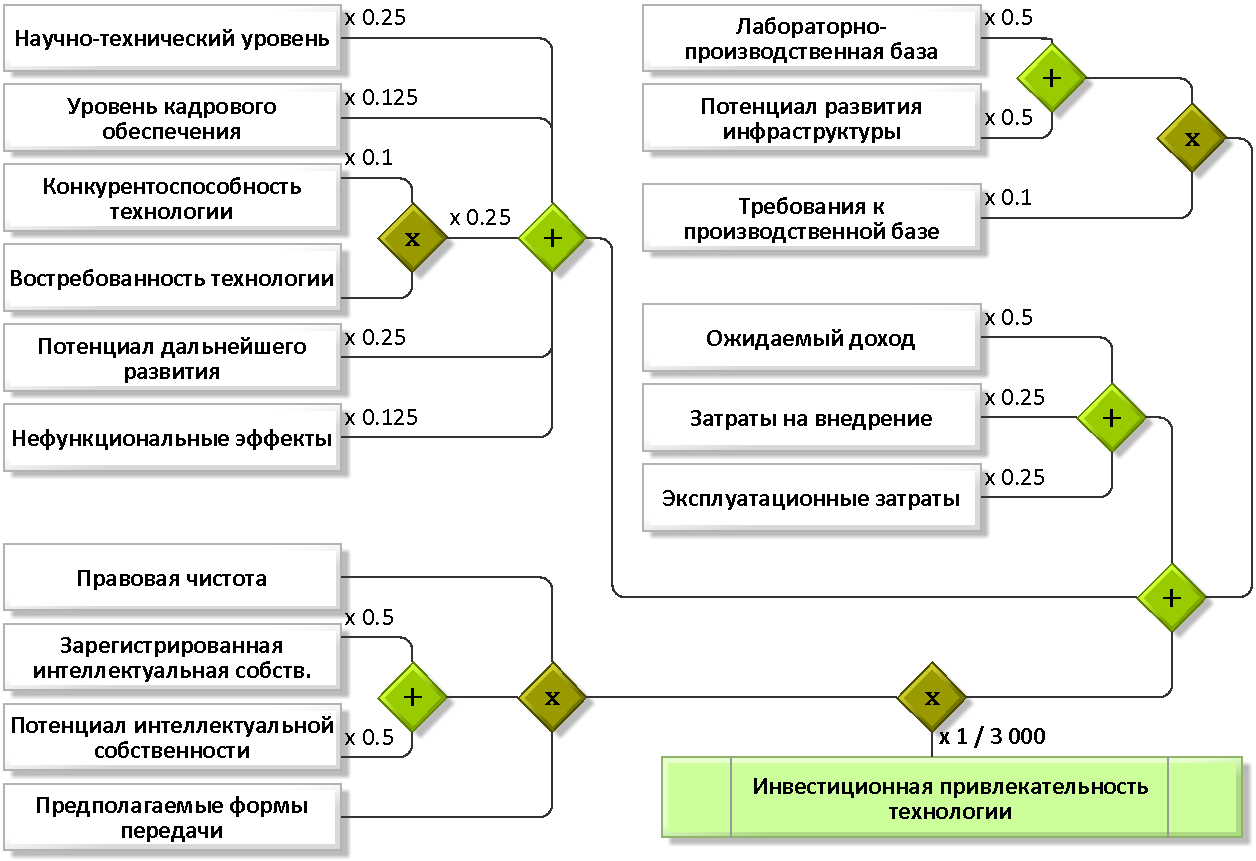
\includegraphics[width=1\linewidth]{./pic/schemeF2}
	\end{center}
\end{frame} %===========================

\begin{frame}{Задача оптимального выбора объектов}
	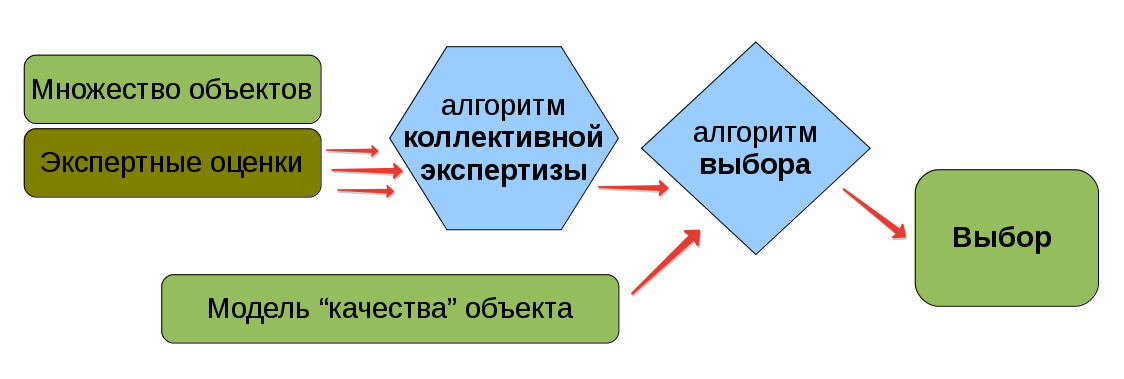
\includegraphics[width=0.8\linewidth]{./pic/globalscheme}
\end{frame} %===========================


\end{document}
